% Recupero Password

Nel caso in cui l'utente avesse smarrito o si fosse dimenticato la password di accesso inserita in fase di registrazione (\S{4}), è possibile cambiarla inserendone una nuova.

\begin{center}
\textsl{ \href{https://dev.d1ay0almkohcfw.amplifyapp.com/passwordDimenticata}{\textbf{https://dev.d1ay0almkohcfw.amplifyapp.com/passwordDimenticata} }}
\end{center}

Per fare ciò, anziché compilare il modulo di Login (\S{5}), l'utente dovrà cliccare sulla voce “Non ti ricordi la password?”

\begin{figure}[H]
\centering
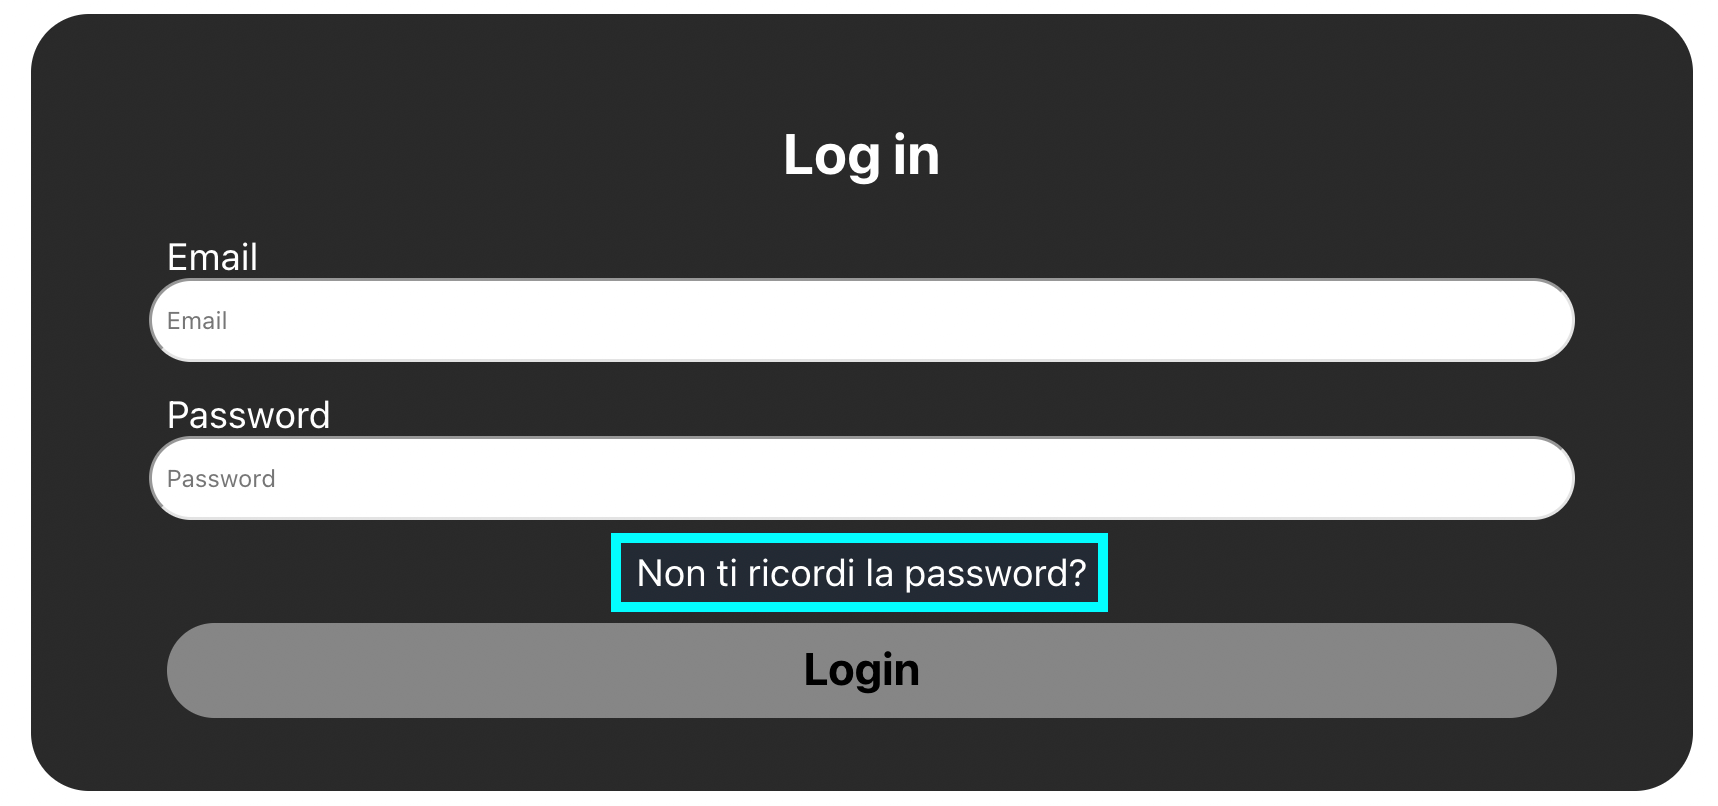
\includegraphics[scale=0.2]{./images/RecuperoPassword/Login.png} 
\caption{Bottone per il recupero password}
\end{figure}

ed inserire l'indirizzo e-mail tramite il quale si vuole verificare l'identità per cambiare la password di accesso.

\begin{figure}[H]
\centering
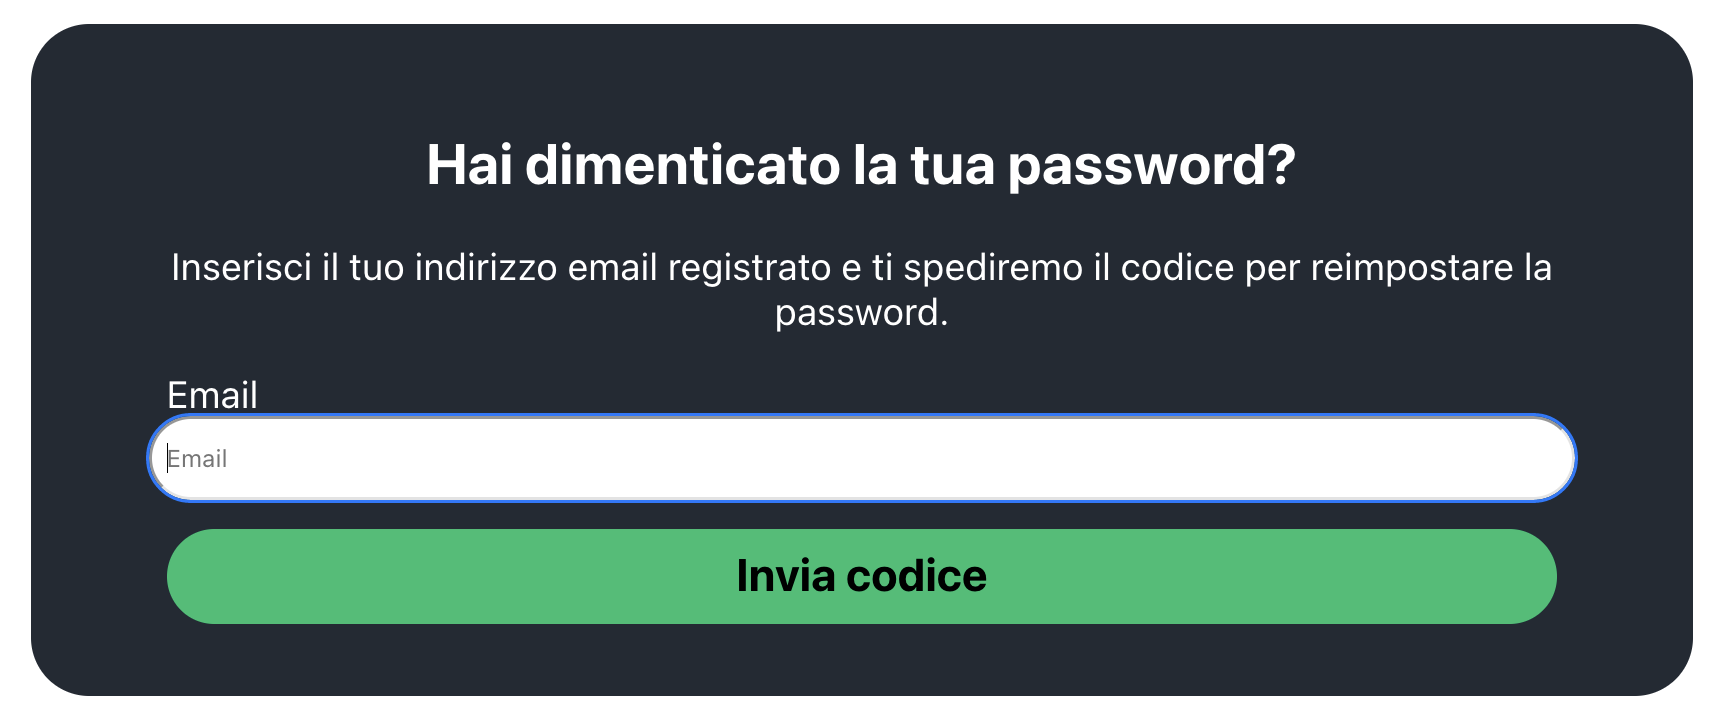
\includegraphics[scale=0.3]{./images/RecuperoPassword/FormRecuperoPwd.png} 
\caption{Form per il recupero password}
\end{figure}

Una volta inserito l'indirizzo e-mail, sarà possibile recuperare la password compilando il form (ossia inserendo l'indirizzo e-mail inserito in fase di registrazione (\S{4})), quindi clicca su “Invia codice”. Riceverai via e-mail un codice numerico di sei cifre, che ti servirà per il prossimo passaggio.

\begin{figure}[H]
\centering
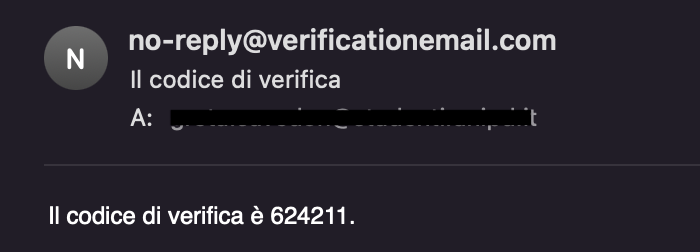
\includegraphics[scale=0.45]{./images/RecuperoPassword/emailRecupero.png} 
\caption{Codice numerico per il recupero password}
\end{figure}

Ora dovrai inserire una nuova password nel form, oltre al codice che avrai ricevuto via e-mail (l'indirizzo e-mail verrà inserito automaticamente).

\begin{figure}[H]
\centering
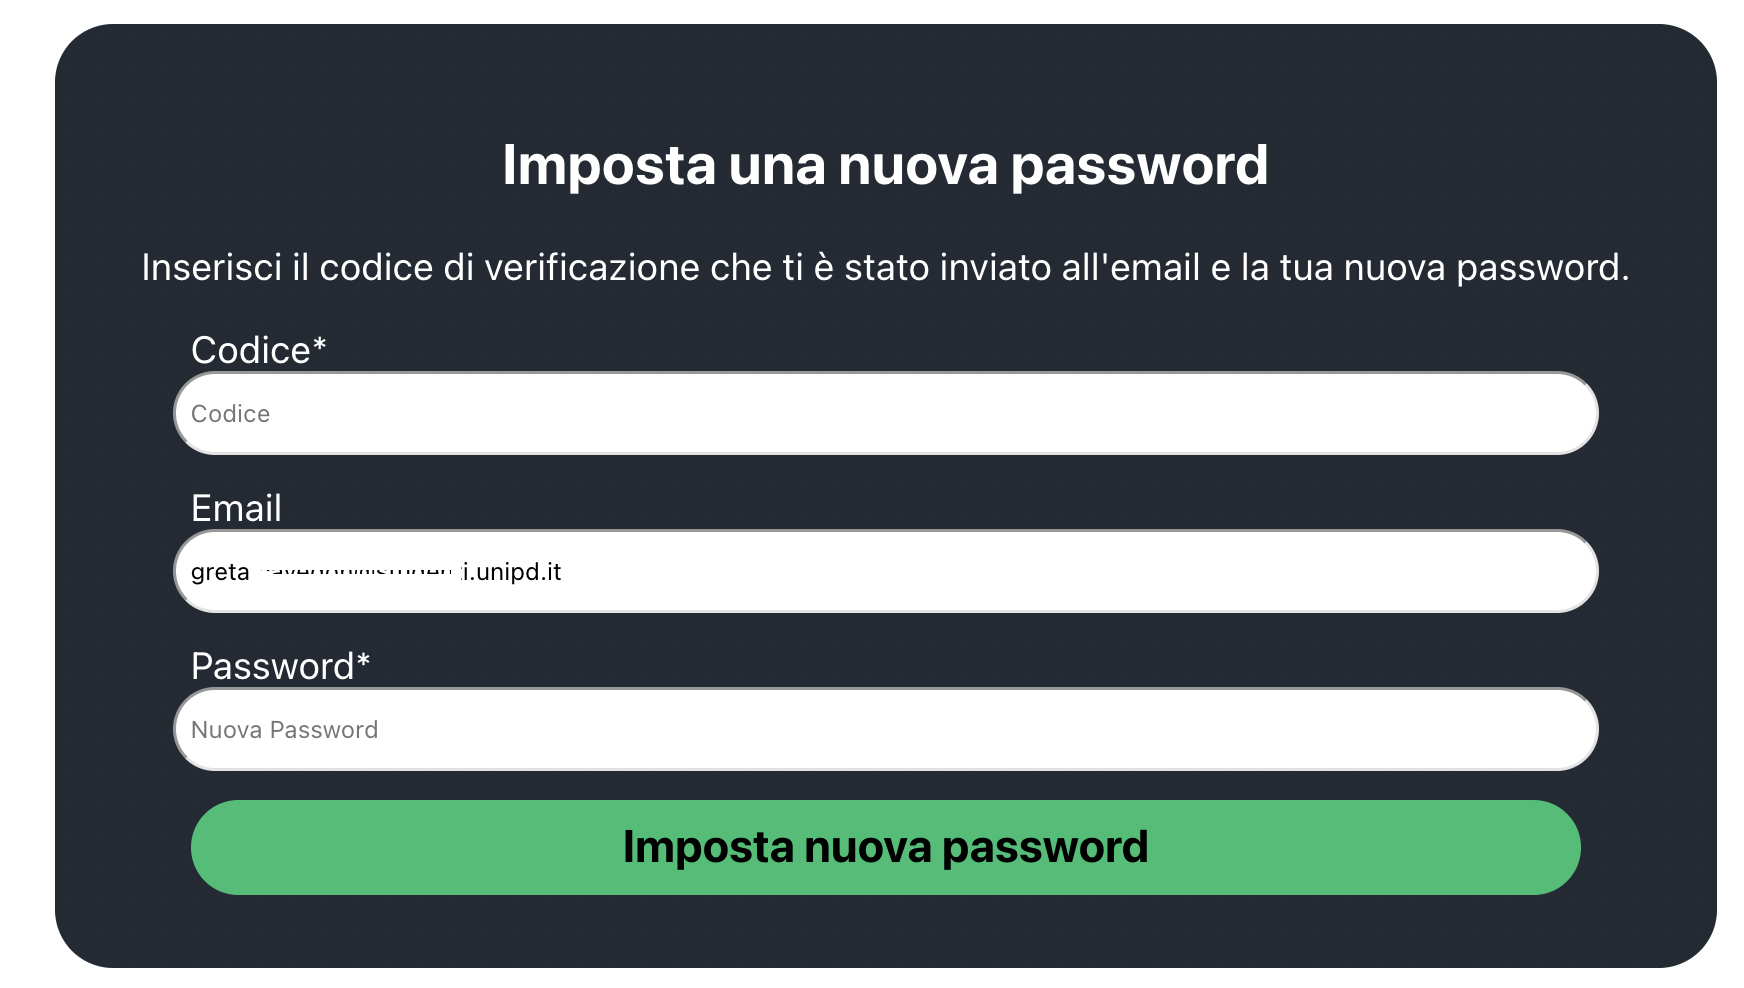
\includegraphics[scale=0.3]{./images/RecuperoPassword/FormNuovaPsw.png} 
\caption{Bottone di registrazione versione desktop}
\end{figure}

Successivamente dovrai cliccare su “\textbf{Imposta nuova password}” e, nel caso il cambio sia andato a buon fine, visualizzare il seguente messaggio:

\begin{figure}[H]
\centering
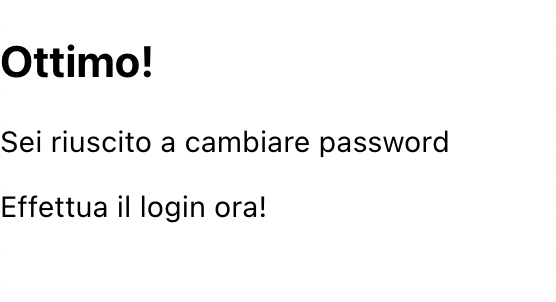
\includegraphics[scale=0.5]{./images/RecuperoPassword/cambioRiusciuto.png} 
\caption{Bottone di registrazione versione desktop}
\end{figure}

Effettua ora il login (\S{5}) per accedere alla tua Area Personale (\S{7}).
